\documentclass{jsarticle}
\usepackage[dvipdfmx]{graphicx}


\newcommand{\argmax}{\mathop{\rm arg~max}\limits}
\newcommand{\argmin}{\mathop{\rm arg~min}\limits}

\begin{document}

\title{ Matrix Profile XIII: Time Series Snippets\\(A New Primitive for Time Series Data Mining)}
\author{}
\date{}
\maketitle

\section{概要}
\subsection{どんな論文?}
Matrix Profileを用いて時系列データから頻繁に表れるような部分時系列(snippets)を抽出

\subsection{似ている手法}
	モチーフ検出、部分時系列クラスタリング、shapeletsなど


\subsection{メリット}
\begin{itemize}
	\item 長い時系列から代表的な(頻繁に表れる)部分時系列を抽出できる
	\item 抽出したsnippetsがどの程度支配的かの割合(論文ではcoverageに対応)を得られる\\
	論文中の例:
	\begin{figure}[h]
		\begin{center}
			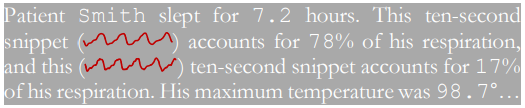
\includegraphics[scale = 0.7]{sleep_example.png}
		\end{center}
		\caption{trainデータの例}
		\label{fig:sleep_example}
	\end{figure}
	\item ノイズに対してロバスト(MPdistを使っているから?)
\end{itemize}

\newpage

\section{手法}
前提知識: matrix profile, MPdist\par
snippetsの長さを$m$に設定する。また、扱う時系列の長さを$n$とする。\newline
\par
\begin{itemize}
	\item snippetsの探索(貪欲法)\\
$Q$ = 値が全てInfのベクトル(長さ$m-n-1$)\\
$C$ = $\emptyset$ (snippetsを格納するリスト)
\begin{enumerate}
	\item 時系列を$n$/$m$等分する(等分された部分時系列を左から$T_1,T_2,\cdots,T_{n/m}$とする)
	\item $T_1,T_2,\cdots,T_{n/m}$のそれぞれについてMPdistベクトルを作成する
	\item for num=1:k
	\begin{itemize}
		\item 各々のMPdistベクトル$D_i$についてProfileAreaを求める \\
		$\mathrm{ProfileArea}_i = \mathrm{sum}(\min({D_i},Q)) $
		\item $j = \argmin_i \mathrm{ProfileArea}_i$を計算し、$C_{num}$に$T_j$を格納\\
		\item $Q = \min(D_i,Q)$に更新
	\end{itemize}
\end{enumerate}
\item coverageの求め方
\begin{itemize}
	\item $T_i$のcoverageは、$T_i$と$Q$で同じ値を取る時間点の割合
\end{itemize}

\end{itemize}

\section{感想・メモ}
\begin{itemize}
\item アルゴリズムはものすごく単純
%\item 計算のボトルネックはMPdistベクトルの計算
\item 貪欲法の部分はもう少し最適化できそうかも(精度的に) 
\item 得られたすべてのsnippetsのcoverageを足すと必ず100\%(以上)になる
%\item shapeletsは部分時系列の頻度でclassificationはできないので、snippetsをうまくclassificationに持っていけたらいい結果が得られる可能性があるかも
\item 計算オーダーが$\mathrm{O}(n^2 \times (n-m)/m)$\\($O(n^2)$:それぞれの部分時系列に対してのMPdistベクトルの計算量、$O((n-m)/m)$:等分された部分時系列の数)\\らしいが、等分された部分時系列の長さは$m$なので、$\mathrm{O}(nm \times (n-m)/m)$ = $\mathrm{O}(n \times (n-m))$ のような気がする・・・\\
($n\gg m$の時,前者と後者のオーダーがそれぞれ$O(n^3)$と$O(n^2)$となり大きな差があるので、どちらが合っているのか要調査)
\end{itemize}
\end{document}